\documentclass[a4paper, 11pt]{article}

\usepackage{graphicx}
\usepackage{subfigure}
\usepackage{amsmath}
\usepackage{color}
\usepackage{subscript}
% Use symbols like degrees
\usepackage{gensymb}
% In case we need to rotate a table
\usepackage{rotating}
% To insert code samples
\usepackage{listings}

% Change margins because article class is too small
\addtolength{\oddsidemargin}{-2cm}
\addtolength{\evensidemargin}{12cm}
\addtolength{\textwidth}{4cm}
\addtolength{\topmargin}{-3cm}
\addtolength{\textheight}{5cm}

% define some colors here if needed
\definecolor{_green}{rgb}{0,0.6,0}
\definecolor{_gray}{rgb}{0.5,0.5,0.5}
\definecolor{_mauve}{rgb}{0.58,0,0.82}
\definecolor{_lyellow}{rgb}{0.1,0.1,0.1}

% code listing settings
\lstset{
  %rulecolor=\color{black},         % if not set, the frame-color may be changed on line-breaks within not-black text (e.g. comments (green here))
  tabsize=2,	                   
  title=\lstname                    % show the filename of files included with \lstinputlisting; also try caption instead of title
  backgroundcolor=\color{white},  % choose the background color;
  language=C++,                     % the language of the code
  basicstyle=\ttfamily\small,       % the size of the fonts that are used for the code 
  aboveskip={1.0\baselineskip},
  belowskip={1.0\baselineskip},
  columns=fixed,
  extendedchars=true,               % lets you use non-ASCII characters; for 8-bits encodings only, does not work with UTF-8
  breaklines=true,                  % sets automatic line breaking
  tabsize=4,                        % sets default tabsize to X spaces
  prebreak=\raisebox{0ex}[0ex][0ex]{\ensuremath{\hookleftarrow}},
  frame=lines,                      % adds a frame around the code (eg. single)
  showtabs=false,                   % show tabs within strings adding particular underscores
  showspaces=false,                 % show spaces everywhere adding particular underscores; it overrides 'showstringspaces'
  showstringspaces=false,           % underline spaces within strings only
  keywordstyle=\color{_mauve},      % keyword style
  commentstyle=\color{_green},      % comment style
  stringstyle=\color{_gray},        % string literal style
  deletekeywords={...},             % if you want to delete keywords from the given language
  otherkeywords={*,...},            % if you want to add more keywords to the set
  numbers=left,                     % where to put the line-numbers;
  keepspaces=true,                  % keeps spaces in text, useful for keeping indentation of code (possibly needs columns=flexible)
  numberstyle=\footnotesize\color{_gray},% the style that is used for the line-numbers 
  stepnumber=1,                     % the step between two line-numbers.
  numbersep=5pt,                    % how far the line-numbers are from the code
  captionpos=t,                     % sets the caption-position bottom(b), top(t)
  escapeinside={\%*}{*)}            % if you want to add LaTeX within your code
}


\begin{document}
\title{Image deformation model in CASToR}
\maketitle

%---------------------------------------------------------------------------------------------------------------------------------------------------------------
\section*{Foreword}

CASToR is designed to be flexible, but also as generic as possible.
Any new implementation should be thought to be usable in as many contexts as possible; among all modalities, all types of data, all types of algorithms, etc.

Before adding some code to CASToR, it is highly recommended to read the general documentation \textit{CASToR\_general\_documentation.pdf} to get a good
picture of the project, as well as the programming guidelines \textit{CASToR\_\_programming\_guidelines.pdf}.
Also, the philosophy about adding new modules in CASToR (\textit{e.g.} projectors, optimizers, deformations, dynamic models, etc) is fully explained in \textit{CASToR\_\_add\_new\_modules.pdf}.
Finally, the doxygen documentation is a very good resource to help understanding the code architecture.

%---------------------------------------------------------------------------------------------------------------------------------------------------------------
\section{Summary}

This HowTo guide describes the image deformation class in CASToR. It provided information about how to use the image deformation models already implemented in CASToR, or how to add a new image transformation class. 

CASToR can manage different type of image-based motion correction, depending on the way the transformation operation is triggered (based on timestamps or specific number of gates and events). This allows to manage several type of motion correction during reconstruction, such as physiological motion (with respiratory and/or cardiac gated acquisition), as well as involuntary body motion. It is assumed that only one type of motion correction can be enabled in a reconstruction, therefore involuntary motion correction cannot be performed with either respiratory or cardiac motion. Simultaneous respiratory and cardiac motion can be performed using a unique set of transformations handling both types of motion.

This guide begins with a description of the preprocessing of the dataset, and the command-line options to enable motion-corrected reconstruction with castor-recon. Section \ref{s_deformation_init} presents the basic for the initialization of a deformation model. The class currently implemented in castor are presented in the following section. The last sections are dedicated to the incorporation of a custom deformation model in CASToR, starting with a presentation of the overall CASToR deformation architecture (section \ref{s_architecture}). Finally, section \ref{s_Add your own deformation model} provides a step-by-step guide that explains how to add a new image deformation by simply adding a new class with few mandatory requirements.
\color{black}

\clearpage
%---------------------------------------------------------------------------------------------------------------------------------------------------------------
\section{Before using any image-based deformation model}
\label{s_prerequisites}

\subsection{Pre-requisites}

Motion management in CASToR differs from the type of motion. The reconstruction of respiratory or cardiac gated acquisitions require a prior reorganization of the events in the dataset into \textit{gates}, as well as the number of events in each gate. The correction of accidental body motion in reconstruction only requires the timestamp of the transformations. Please have a look at section 7 of the general documentation for a description of how dynamic datafiles are handled by CASToR for each type of motion.


\subsubsection{Motion correction for gated acquisition (-rm, -cm)}

Gated-acquisition are usually performed to adress physiological motion such as respiratory and cardiac motions. Due to the cyclic nature of these motions, the CASToR implementation requires a specific organization of the datafile. The implementation of image-based correction for these types of motion assumes the elements of the raw datafile (list-mode lines of response, or histogram bins) has previously been sorted into different subsets (\textit{gates}), as described in section 7 of the general documentation file. Each \textit{gate} corresponding to a specific phase of the motion surrogate (e.g, to a respiratory or cardiac phase/amplitude).

The command-line options to enable motion-correction for gated acquisitions depend on the nature of motion. The \textit{-rm}, \textit{-cm} command-line options allow to set up a deformation model for respiratory or cardiac motion-corrected reconstruction respectively. These option must be used along with the \textit{-g} option, which provides a configuration file containing the number of gates and the number of events in each gates of the dataset. Section \ref{s_deformation_init} describes how to set the deformation model with \textit{-rm} or \textit{-cm}.

\subsubsection{Motion correction for involuntary patient motion (-im)}

The implementation of image-based body motion correction requires the timestamp of the transformations to correct the data. During image reconstruction, the transformation operations will be performed when the timestamp of the event is greater than the next timestamp of the deformation. To set up a deformation model for this kind of motion, the command-line option \textit{-rm} must be used. The timestamp of the transformations must be provided from a file with 
the \textit{-g} option, as described in section 7 of the general documentation. The next section of the document describes how to set the deformation model with \textit{-im}.




\clearpage
\section{Deformation model initialization}
\label{s_deformation_init}

A deformation module can be enabled in order to perform image-based transformations. The \textbf{-rm}, \textbf{-cm} and \textbf{-im} command line options (for respiratory, cardiac and involuntary patient motion correction respectively) must be used to provide the image deformation information. Depending on the model, the initialization can be performed with a set of parameters, or with a configuration file, using the following syntaxes: 

\verb| -rm model,option1,option2,...|
\verb| -rm model:path/to/configuration/file|

The first line corresponds to initialization with a set of options (such as transformation parameters). The alias of the deformation model must be written first, followed by the parameters, separated by commas.
The second line corresponds to an initialization with a configuration file containing and associated parameters. The alias of the deformation model must be written first, followed by a semi-colon, and the path to the configuration file.


\paragraph{Transformation vectors:} During image reconstruction, the image-based motion correction operations will be applied when the code reach a trigger computed from the number elements in each gate (for gated dataset), or from a timestamp (for patient motion). These operations requires a set of \textit{forward} transformations (from a reference position, corresponding to the position in which the images will be reconstructed, to any other position (gate or patient motion time subset) of the dataset), and \textit{backward} transformations (from any position to the reference position). The reference position can be any of the gate (or part of data corresponding to a time subsets in the case of accidental motion). 

Figure \ref{fig_transformation} illustrates the transformations required for motion correction. For gated dataset (fig. \ref{fig_transformation_a}), both \textit{forward} and \textit{backward} transformations must be provided between the reference position and each gate position. In the case one gate corresponds to the reference position, identity parameters must be provided. Likewise, for timestamp based motion, transformation parameters must be provided for each subset of data between two timestamps.


\begin{figure} [h]
  \centerline
  {
    \subfigure[Gated based motion]{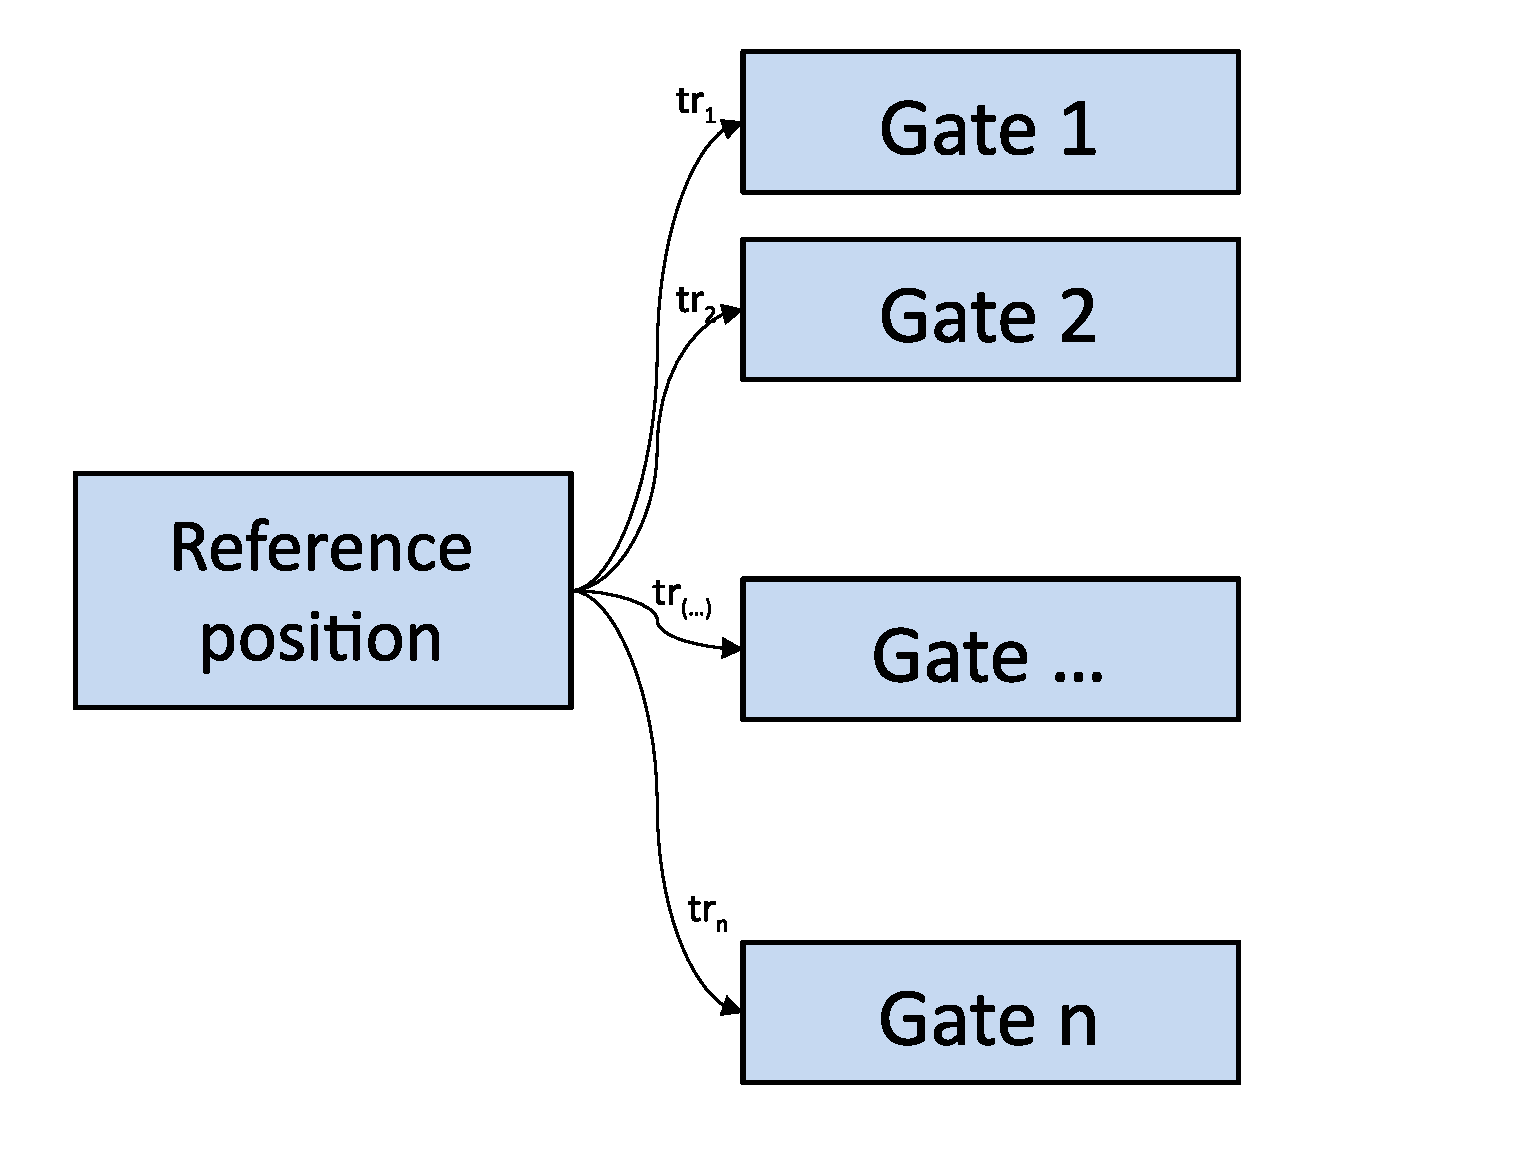
\includegraphics[width=0.49\columnwidth]{./figures/deformation_gating.eps}
    \label{fig_transformation_a}}
    \subfigure[Timestamp based motion]{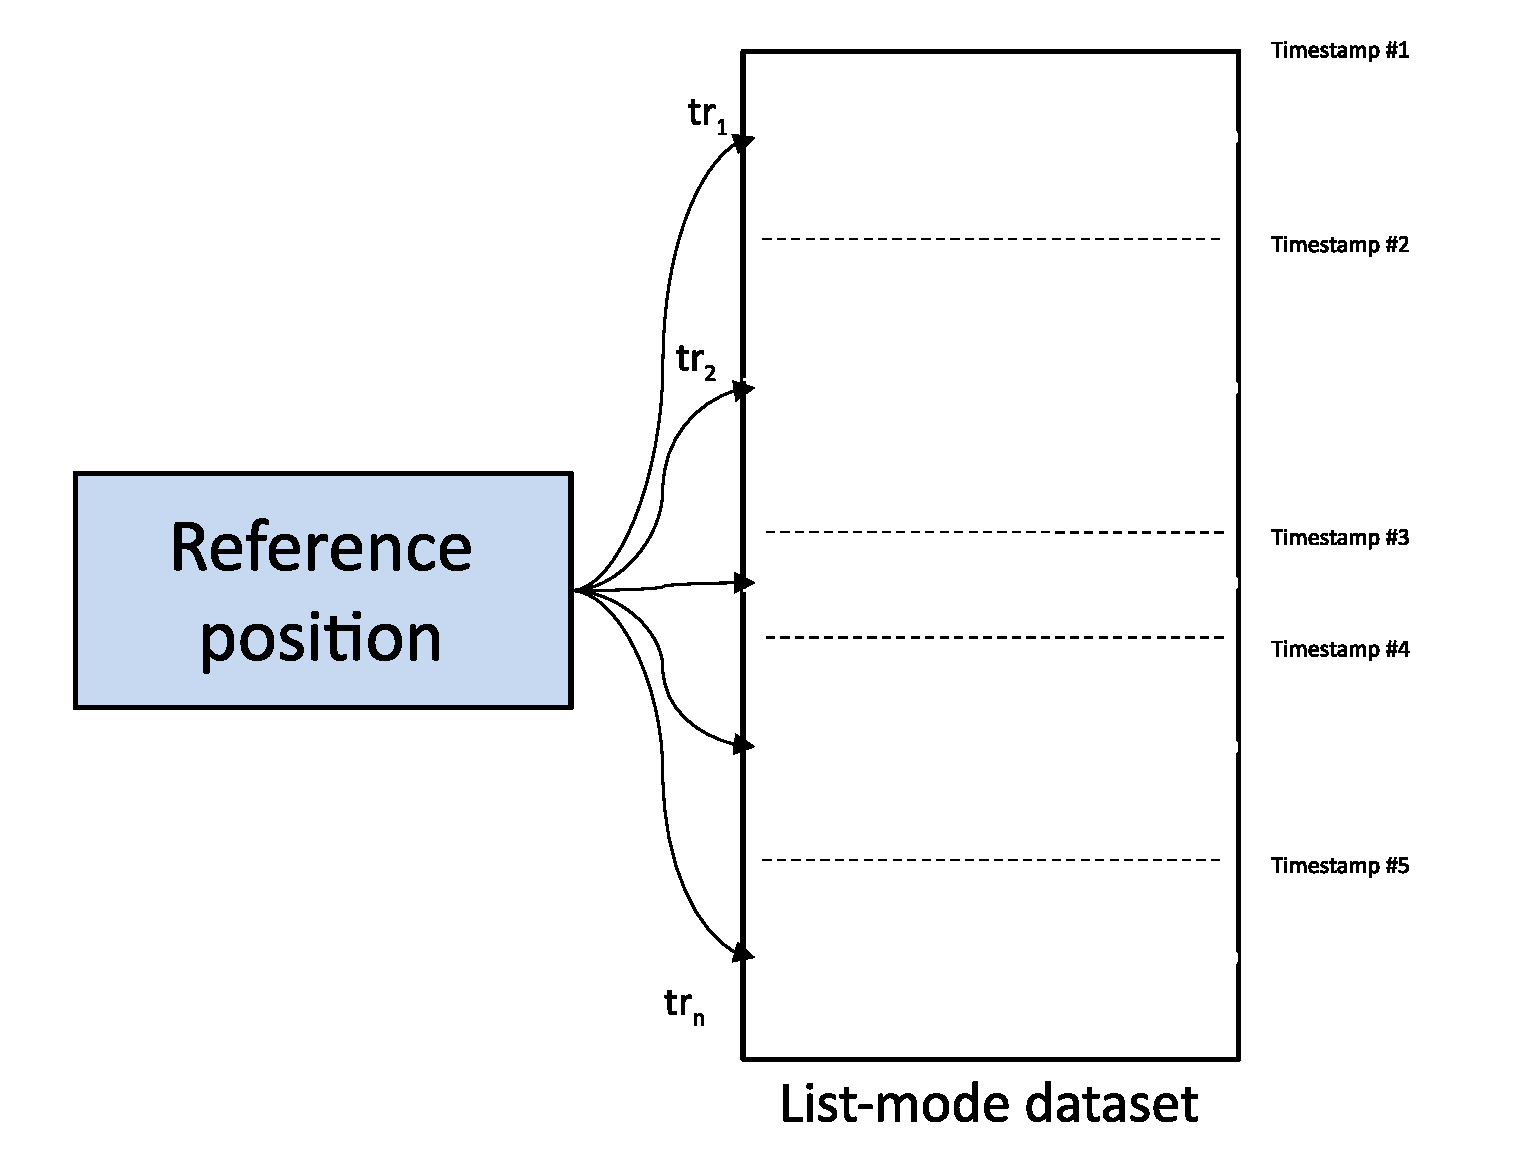
\includegraphics[width=0.49\columnwidth]{./figures/deformation_timestamp.eps}
    \label{fig_transformation_b}}
  }
  \caption{Definition of \textit{forward} (left arrows) and \textit{backward} (right arrows) transformations between the gates of the dataset}
  \label{fig_transformation}
\end{figure}


This option allows to initialize a rigid or elastic deformation model and associated parameters (see details in section \ref{section_Meta-data command line options}). CASToR contains a rigid (\textbf{deformationRigid}, section\ref{ss_rigid}) in order to perform image-based transformation, as described below. 


\clearpage
\section{Implemented deformation model}
\label{s_implemented_model}

This section lists the deformation model implemented in CASToR. Currently, only a rigid deformation model is implemented. Details about the available deformation models and information regarding their initialization can be displayed using the command  \textbf{-help-motion}. 

\subsection{deformationRigid:}
\label{ss_rigid}

This class uses rigid deformations whose transformation vectors are parameterized by 3 translations and 3 rotations. As most modules, it can be initialized from the command-line options: 

\bigskip
\verb| -im deformationRigid,tx1,ty1,tz1,ra1,rb1,rc1,tx2,ty2,tz2,ra2,rb2,rc2,...| \\


where tx, ty, tz represents the translations along the different axis, and ra, rb, rc represents the 3 rotations to perform along specific axis (x, y, and z) by default.

\bigskip
Or using a configuration file :
\bigskip
\verb| -im deformationRigid:/path/to/conf/file.txt|
\bigskip

The listing below displays an example of configuration file. Each transformation parameters (3 translations (mm), 3 rotations (degrees)) must be entered on a separate line. 

The \textit{Rotation\_convention} parameter defines the axis for the rotation of the 3 angles according to the different conventions (\textit{XYZ}, \textit{ZYX}, \textit{XYX}, etc.. default is \textit{XYZ}). 

The forward and backward deformations will be automatically computed from the parameters provided by \textit{Transformation\_parameters}. By default, the transformation parameters must correspond to the transformation between the reference position \textit{i} to each subset (or gate), as illustrated in figure \ref{fig_transformation}. 

One can also provide parameters from the position \textit{i} to the next position \textit{i+1} (usually assuming that the first gate/subset is the reference). In this case, the \textit{Transformation\_mode} parameter must be set to 1. 

\begin{lstlisting}[label={list_rmotion_conf},caption= Example of a configuration file for rigid transformation.]

// Parameters for rigid deformation (tx, ty, tz, rx, ry, rz)
Transformation_parameters:
0,0,0,0,0,0
1,2,-3.5,-3.5,-2,4.5
3,-0.5,-4.25,3.75,-2,4.25
1,2,1.5,-0.75,-3.5,-3
-0.75,0.5,-2,-4,-3.25,-3
-0.5,3,2.5,1.75,-0.5,-3.5

// Convention of rotation (any combination of XYZ axis)
Rotation_convention: XYZ

// Parameters computation:
// 0: Each line of parameters represent the actual deformation in comparison with the reference position
// 1: Each line of parameters represent the deformation with the previous position. 
Transformation_mode: 0

\end{lstlisting}   



%\subsection{deformationElastic:} 
%\label{ss_elastic}
%This class implements non-rigid deformation using the \textit{Elastix} library\cite{Elastix}. Elastix is a program for image registration which supports many registration methods and various transformation models. Most part of the Elastix code requires the Insight Segmentation and Registration Toolkit (ITK), so CASToR must be first compiled with both ITK and Elastix in order to be used.


%\color{red}
%\paragraph{Compilation instructions:} TODO Fred (detailler la compilation avec ITK et Elastix)


%\paragraph{Initialization:} TODO Fred (detailler la configuration et l'utilisation de deformationElastic)
%\color{black}


\clearpage
%---------------------------------------------------------------------------------------------------------------------------------------------------------------
\section{The image deformation architecture}
\label{s_architecture}

The image deformation part of the code is based on 2 main classes: \textit{oDeformationManager} and \textit{vDeformation}. The main program will instantiate and initialize the \textit{oDeformationManager}, and during the iterative reconstruction process, the \textit{oDeformationManager::PerformDeformation()} function will apply the required deformations on the different image matrices when the event counter hits a trigger (a certain number of events in the case of gated dataset, or a certain timestamp for involuntary patient motion). The various steps of application of the deformations on the different image matrices of the algorithm (forward image containing the image to project, backward image containing the correction factors, etc...) is natively managed by the \textit{vDeformation} mother class, so that the developper doesn't need to handle this in his deformation class. 

The \textit{vDeformation} class only requires that the child implements the \textit{ApplyDeformations()} function, which will perform the deformation on an input image matrix, and recover the result in an output image matrice, both passed in argument. Please have a look to the section \ref{section_Add your own deformation model} for more help about the deformation model implementation itself.

It is worthy to note that the deformation process itself is NOT multithreaded, therefore a synchronization of the threads will be performed before each image deformation. This is to limit the RAM requirements on some image matrices which should not be multithreaded a-priori. 

Regarding the sensitivity image of list-mode reconstruction, the algorithm will generate an image corresponding to the reference position using the \textit{Forward} and \textit{Backward} transformations. The algorithm will simply loop on the total number of transformations, generate a reference image for each set of \textit{Forward} and \textit{Backward} transformation, and average all these images to get a standard reference sensitivity image.


\clearpage
%---------------------------------------------------------------------------------------------------------------------------------------------------------------
\section{Add your own deformation model}
\label{s_Add your own deformation model}

\subsection{Basic concept}

To add a new image-based deformation module, the user only has to build a specific class that inherits from the abstract class \textit{vDeformation}. Then, one just has to implement a set of pure virtual functions for the initialization and application of the model. Please refer to the \textit{CASToR\_\_add\_new\_modules.pdf} guide in order to fill up the mandatory parts of adding a new module; namely the auto-inclusion mechanism, the interface-related functions and the management functions. Right below are some instructions to help you fill the specific pure virtual projection functions of deformation model.

\bigskip
To ease the implementation, a template class is provided in the source code and already implements all the squeleton. Basically, one will have to change the name of the class and fill the related functions up in his own code. The actual files are \textit{include/image/iDeformationTemplate.hh} and \textit{src/image/iDeformationTemplate.cc} and are actually already part of the source code.

\subsection{Implementation of the deformation functions}

Several mandatory functions should be implemented (or return an error by default) in a new deformation model class :

\begin{description}
\item \textbf{ShowHelp()}: Simply output some help and guidance to describe what the deformation model does and how to use it.
\item \textbf{ReadAndCheckOptionsList()}: Implement here the reading of any options specific to this deformation model passed through the argument \texttt{const string\& a\_listOptions}. The user can make use of the \textit{ReadStringOption()} function to parse the list of parameters. If the function is not mandatory (e.g initialization of the model using a file is required tather than with command-line parameters), just send an error message and return 1.
\item \textbf{ReadAndCheckConfigurationFile()}: Implement here the reading of any configuration file specific to this deformation model, passed through the argument \texttt{const string\& a\_fileOptions}. The user can make use of the \textit{ReadDataASCIIFile()} function to read data from a file. If the function is not mandatory (e.g initialization of the model using command line options is required rather than with a file), just send an error message and return 1.
\item \textbf{CheckParameters()}: Use this function to check if the private parameters of your class have correctly been initialized. It might be a good idea to initialize all private parameters in the constructor with default erroneous value to properly check their initialization.
\item \textbf{Initialize()}: Use this function to Instanciate/Initialize any member variables/arrays after the parameters have been checked in the previous function.  
\item \textbf{ApplyDeformation()}: The deformation model must be implemented here, with the help of any private functions if required. This function is described in the pseudocode below. This function has 4 arguments:
\begin{description}
\item[\texttt{ap\_inputImage}]: vector containing the input image to deform
\item[\texttt{ap\_outputImage}]: vector in which the transformed image must be recovered
\item[\texttt{a\_direction}]:  integer which indicates the direction of the deformation to perform, i.e: 

\texttt{FORWARD\_DEFORMATION} (from the reference position to the \texttt{a\_defIdx} position), 

\texttt{BACKWARD\_DEFORMATION} (from the \texttt{a\_defIdx} position to the reference position). 

The integers \texttt{FORWARD\_DEFORMATION} and \texttt{BACKWARD\_DEFORMATION} are defined in the beginning of vDeformation.hh as macros
\item[\texttt{a\_defIdx}]: defines the index of the transformation
\end{description}

All information and the tools needed to implement these functions are fully described in the template source file \textit{src/projector/iDeformationTemplate.cc}, so please refer to it.

\end{description}




\begin{lstlisting}[label={sample},caption= Description of ApplyDeformations function.]

int iDeformationTemplate::ApplyDeformations(FLTNB* ap_inputImage, 
                                            FLTNB* ap_outputImage, 
                                            string a_direction, 
                                            int a_defIdx)
{
  // This function is an implementation of the pure virtual mother function. The actual deformation should be implemented here, with the help of any private functions if required

  // IMAGE DIMENSIONS:
  // For code efficiency and readability, the spatial index of a voxel is a cumulative 1D index. 
  // That is to say, given a voxel [indexX,indexY,indexZ],
  // its cumulative 1D index is computed by 'index = indexZ*nbVoxXY + indexY*nbVoxX + indexX'.

  // The image dimensions can be recovered from the mp_ImageDimensionsAndQuantification class
  // Total number of voxels         : 
  mp_ImageDimensionsAndQuantification->GetNbVoxXYZ()
  // Number of voxels in a slice    : 
  mp_ImageDimensionsAndQuantification->GetNbVoxXY()
  // Number of voxels on the X-axis : 
  mp_ImageDimensionsAndQuantification->GetNbVoxX()
 

  // Any error should return a value >0.
  
  return 0;
}
\end{lstlisting}


\clearpage
\section{Meta-data command line options}
\label{section_Meta-data command line options}
List of the different set of options related to image-based deformations :
\begin{itemize}
\item \textbf{-g} \textit{file}: Give a text file defining the dynamic data splitting (due to respiratory/cardiac gating or involuntary patient motion correction).
      The file should contain the some of the following keywords :
\begin{description}
\item \texttt{nb\_respiratory\_gates}: number of respiratory gates in the data
\item \texttt{nb\_events\_respiratory\_gates}: enter the number of events within each gate, separated by commas. If the data contains several frame (dynamic acquisition), the data splitting of each frame should be entered on a new line (1 line by frame).
\item \texttt{nb\_cardiac\_gates}: number of cardiac gates in the data
\item \texttt{nb\_events\_cardiac\_gates}: enter the number of events within each gate, separated by commas. If the data contains several frame (dynamic acquisition), the data splitting of each frame should be entered on a new line (1 line by frame).
\item \texttt{nb\_involuntary\_motion\_triggers}: number of involuntary patient motion triggers in the data
\item \texttt{list\_involuntary\_motion\_triggers}: enter the timestamp of each transformation, separated by commas. No specific nomenclature is required for dynamic acquisitions (data containing several frames). However, if the data contains several bed positions, the data splitting of each bed should be entered on a new line.
\item \texttt{duration\_gate}: (optional) enter the duration (seconds) of each gate, separated by commas. If the data contains several frames (dynamic acquisition), the gate durations within each frame should be entered on different line (1 line by frame).
\end{description}
\item \textbf{-rm} \textit{param}: Give the deformation to be used for respiratory motion correction, along with a configuration file (deformationModel:file), or the list of parameters associated to the deformation model (deformationModel,param1,param2,...).
\item \textbf{-cm} \textit{param}: Give the deformation to be used for cardiac motion correction, along with a configuration file (deformationModel:file), or the list of parameters associated to the deformation model (deformationModel,param1,param2,...).
%\item \textbf{-rcm} \textit{param}: Give the deformation to be used for dual gating motion correction (both respiratory and cardiac), along with a configuration file (deformationModel:file), or the list of parameters associated to the deformation model (deformationModel,param1,param2,...).
\item \textbf{-im} \textit{param}: Give the deformation to be used for patient motion correction, along with a configuration file (deformationModel:file), or the list of parameters associated to the deformation model (deformationModel,param1,param2,...).
\end{itemize}


%---------------------------------------------------------------------------------------------------------------------------------------------------------------
%---------------------------------------------------------------------------------------------------------------------------------------------------------------
%---------------------------------------------------------------------------------------------------------------------------------------------------------------
%          R E F E R E N C E S
%---------------------------------------------------------------------------------------------------------------------------------------------------------------
%---------------------------------------------------------------------------------------------------------------------------------------------------------------
%---------------------------------------------------------------------------------------------------------------------------------------------------------------
\bibliographystyle{IEEEtran} 
%\bibliographystyle{apalike} 
\bibliography{CASToR_general_documentation}

\end{document}
